\documentclass[main]{subfiles}

\begin{document}

\section{Chapter 1: Representing Data}

\begin{itemize}
    \item Categorical data: categories / anything you can't take $\mu$ of
    \item Quanitative data: numerical / anything you can take $\mu$ of
\end{itemize}

\subsection{Describing Graphs/Distributions}
\begin{itemize}
    \item \textbf{S}hape: symmetrical or skewed; unimodal, bimodal, or multimodal
        \subitem 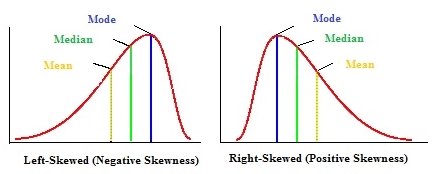
\includegraphics[scale=0.7]{skewed_distribution}
    \item \textbf{O}utliers: visual identify, or: smaller than $Q_1 - 1.5 \times IQR$ or greater than $Q_3 + 1.5 \times IQR$
    \item \textbf{C}enter
    \item \textbf{S}pread
\end{itemize}

\subsection{Measures of center and spread}
\begin{tabular}{ | p{3cm} || p{3cm} | p{3cm} | }
    \hline
    \textbf{\textit{Type}} & \textbf{Resistant} & \textbf{Non-resistant} \\
    \hline
    \textbf{Center} & Median & Mean ($\mu$)\\
    \hline
    \textbf{Spread} & IQR ($Q_3 - Q_1$) & Range \newline Std. deviation ($\sigma$) \\
    \hline
\end{tabular}
\\~\\
\noindent\hyperlink{toc}{Back!}
\newline\hrule

\section{Chapter 2: Distributions of Data}
\begin{itemize}
    \item z-score: \[z = \frac{x - \mu}{\sigma}\]
    \item OGIVE! (cumulative frequency graph)
    \item $N(\mu, \sigma)$ is the Normal distribution function
    \item Sums of independent Normal distributions are still Normally distributed
\end{itemize}

\subsection{Transformation of data}
\begin{tabular}{ | p{3.2cm} || p{2.5cm} | p{2.5cm} | p{2.5cm} | p{2.5cm} | }
    \hline
    \textbf{\textit{Type}} & \textbf{Center}, \newline i.e. $\mu$ & \textbf{Location}, \newline i.e. percentile & \textbf{Spread}, \newline i.e. $\sigma$ & \textbf{Shape}, \newline i.e. $N$ \\
    \hline
    \textbf{Add \newline subtract $a$} & $+\:a$\newline$-\:a$ & $+\:a$\newline$-\:a$ & No change & \multirow{2}{*}{No change} \\
    \cline{1-4}
    \textbf{Multiply \newline divide by $b > 0$} & $\times\:b$\newline$\div\:b$ & $\times\:b$\newline$\div\:b$ & $\times\:b$\newline$\div\:b$ & \\
    \hline
\end{tabular}
\\~\\
\noindent\hyperlink{toc}{Back!}
\newline\hrule

\section{Chapter 3: Correlation and LSRL}
\subsection{Scatterplot}
\begin{itemize}
    \item 2 quantitative vars on same individuals
        \subitem Explanatory var: $x$
        \subitem Response var: $y$
    \item Describe:
        \subitem \textbf{F}orm: linear, curved
        \subitem \textbf{O}utliers: visual identify
        \subitem \textbf{D}irection: positive, negative
        \subitem \textbf{S}trength: weak, moderate, strong
\end{itemize}

\noindent\hyperlink{toc}{Back!}
\newline\hrule

\subsection{LSRL (least-squares regression line)}
\begin{itemize}
    \item \textbf{Include units!}
    \item $\hat{y} = a + bx$ where:
        \subitem $\hat{y}$ is the predicted y
        \subitem $a$ is the y-intercept
        \subitem $b$ is the slope
        \subitem \textbf{Script:} the slope $b = ...$ tells us that the \{response variable\} is predicted to go up/down by $|\:b\:|$ for each \{explanatory variable\}.
        \subitem \textbf{Script:} the y-intercept $a = ...$ is the predicted \{response variable\} at 0 \{explanatory variable\}.
    \item Outputs of LSRL:
        \subitem $r$ is the correlation coefficient
        \subitem $r^2$ is the coefficient of determination
        \subsubitem $r$ or $r^2$ cannot support/deny linearity
        \subitem \textbf{Script:} About $r^2$\% of the variation in \{response var.\} is accounted for by the LSRL relating \{response var.\} to \{explanatory var.\}.
        \subitem \textbf{Script:} When using the LSRL with $x = $ \{explanatory var.\} to predict $y = $ \{response var.\}, we will typically be off by about $S_{residuals}$ \{response var.\}.
    \item $Residual = y - \hat{y}$
        \subitem Positive (+) residual: predicted value \textit{underestimated} observed value
        \subitem Negative (-) residual: predicted value \textit{overestimated} observed value
        \subitem Residual plot: data is linear if plot has no structure, looks random, and doesn't deviate too much
\end{itemize}

\noindent\hyperlink{toc}{Back!}
\newline\hrule

\section{Chapter 4: Observational Studies and Experiments}
\begin{itemize}
    \item Observational study: purely observational, \textbf{no treatment!}
    \item Experiment: \textbf{yes treatment!}
\end{itemize}

\subsection{Types of sampling}
\begin{itemize}
    \item Simple random sample (SRS)
    \item Stratified random sample
    \item Clustered random sample
        \subitem 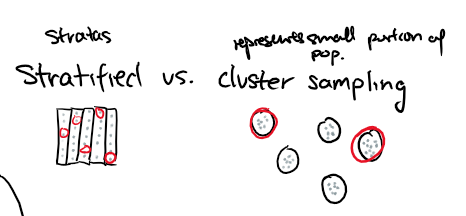
\includegraphics[scale=0.8]{stratifiedcluster_sampling}
    \item Convenience sample (\textbf{\textit{BAD!!!}})
\end{itemize}

\noindent\hyperlink{toc}{Back!}
\newline\hrule

\subsection{Types of bias}
\begin{itemize}
    \item Selection bias: fix by random sampling
        \begin{itemize}
            \item Undercoverage: some groups aren't well represented (i.e. conservative newspaper)
                \subitem Overcoverage: some groups are too well represented
            \item Non-response: some groups can't respond (i.e. online survey)
            \item Voluntary response (i.e. call-in survey)
        \end{itemize}
    \item Response bias: fix by better/less awkward question
        \begin{itemize}
            \item Wording of question: leading question
            \item Social desirability: people don't admit to socially/politically incorrect or illegal things
        \end{itemize}
    \item \textit{Natural variability/sampling error}: fix by increasing $n$
\end{itemize}

\noindent\textbf{Effects of bias:}
\begin{itemize}
    \item Underestimate
    \item Overestimate
\end{itemize}

\noindent\hyperlink{toc}{Back!}
\newline\hrule

\section{Chapter 5: Probability}
\begin{itemize}
    \item $P(A)$: probability of event A occurring
    \item $P(A')$ or $P(A^c)$: probability of event A \textit{not} occurring
    \item $P(A \cup B) = P(A) + P(B) - P(A \cap B)$: probability of A \textit{or} B occurring
    \item $P(A \cap B)$: probability of A \textit{and} B occurring
    \item $P(A | B)$: probability of event A occurring \textit{given that} event B occurred.
    \item Check \textbf{mutually exclusive}:
        \[P(A \cap B) = 0, \;\;if\; \textrm{mutually exclusive}\]
    \item Check \textbf{independence}:
        \[P(A) = P(A|B) = P(A|B') = \frac{P(A \cap B)}{P(B)}, \;\;if\; \textrm{independent}\]
\end{itemize}

\noindent\hyperlink{toc}{Back!}
\newline\hrule

\section{Chapter 6: Random variables, binomial, geometric}

\subsection{Discrete random variable}
\begin{itemize}
    \item \textit{1-Var Stats}
    \item Sums of independent Normal random variables are still Normally distributed
\end{itemize}

\subsection{Binomial distributions (identified by probability of success $p$, trials $n$)}
\begin{itemize}
    \item BINS: binary outcomes, independence, fixed $n$, same $p$ for all trials
    \item $binompdf(n, p, x) = P(X = x)$
    \item $binomcdf(n, p, x) = P(X \leq x)$
\end{itemize}

\subsection{Geometric distributions (identified by probability of success $p$)}
\begin{itemize}
    \item BITS: binary outcomes, independence, interested in trials before first success, same $p$ for all trials
    \item $geometpdf(p, x) = P(X = x)$
    \item $geometcdf(p, x) = P(X \leq x)$
\end{itemize}

\noindent\hyperlink{toc}{Back!}
\newline\hrule

\subsection{Combining Random Variables}
\begin{itemize}
    \item Add: $S = X + Y$
        \subitem $\mu_{S} = \mu_X + \mu_Y$
        \subitem $\sigma_S = \sqrt{\sigma_X^2 + \sigma_Y^2}$
    \item Subtract $D = X - Y$
        \subitem $\mu_{D} = \mu_X - \mu_Y$
        \subitem $\sigma_D = \sqrt{\sigma_X^2 + \sigma_Y^2}$
    \item Multiply $P = a \times X$
        \subitem $\mu_{P} = a \times (\mu_X)$
        \subitem $\sigma_P = \sqrt{a \times (\sigma_X^2)}$
\end{itemize}

\noindent\hyperlink{toc}{Back!}
\newline\hrule

\section{Chapter 7: Sampling Distributions}
\begin{itemize}
    \item Statistic $\rightarrow$ Sample
    \item Parameter $\rightarrow$ Population
    \item Conditions
        \subitem Proportion: 
            \subsubitem Large counts: $np \geq 10$ or $n(1 - p) \geq 10$
            \subsubitem 10\% condition: $n \leq 0.1N$
        \subitem Means: 
            \subsubitem Central limit theorem (CLT): $n \geq 30$
            \subsubitem 10\% condition: $n \leq 0.1N$
    \item Figure out using formula sheet:
        \subitem Proportions: $\mu_{\hat{p}}$ and $\sigma_{\hat{p}}$
        \subitem Means: $\mu_{\bar{x}}$ and $\sigma_{\bar{x}}$
    \item Use $normalcdf$ with above values as $\mu$ and $\sigma$ to find probability
\end{itemize}

\noindent\hyperlink{toc}{Back!}
\newline\hrule

\end{document}